\chapter{Fundamentals} % and theoretical background (BASICS)
\label{ch:fundamentals}

\section{Surface representations}
\label{sec:surface_representations}

CAD and CAM software use several different representations for final and intermediate geometric parts like cutter geometries, the manufactured workpiece or the current machining state.
Tukora provides a comprehensive list with sketches and descriptions of the most commonly used representations \cite{virtual_machining_review}. These will be discussed in this section. 

\begin{description}
	\item[Vector clipping] \hfill \\
	Vector clipping is mainly used in CAE to verify the correctness of a generated (C)NC program before it is run on an actual milling machine and has been first described by Chappel \cite{vector_clipping} in 1983.
	The method requires the geometries of the final workpiece as well as the stock (\ie the original piece of material it has been cut out of).
	Initially, points on the final workpiece are calculated together with surface normals (\ie a point cloud) where the normals are not necessary of unit length but long enough to reach the surface of the stock.
	To simulate the manufacturing process, the cutter is moved over this point cloud and the vectors attached to the points are clipped by the moving cutter (\cf figure \ref{fig:vector_clipping}).
	Tukora compares this method to a lawn mower, which cuts the grass (\ie the normal vectors) towards the ground (\ie the final workpiece).
	After cutting has completed, the lengths of the remaining vectors indicate the local error of the (C)NC program.
	Vectors with positive lengths mark areas where too less material has removed and vice versa.
	The vector lengths are finally used to color the final workpiece where the color indicates the severity of the machining error. 
	
	\begin{figure}[h]
		\centering
		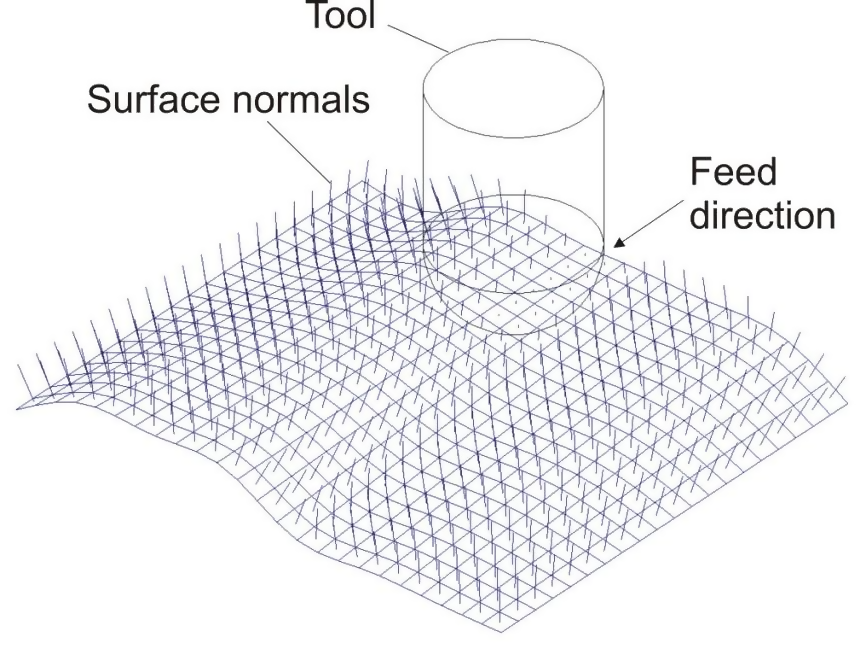
\includegraphics[width=0.5\textwidth]{images/vector_clipping}
		\caption{
			The vector clipping method as described by Chappel \cite{vector_clipping}.
			Image by Tukora \cite{virtual_machining_review}.
		}
		\label{fig:vector_clipping}
	\end{figure}
	 
	\item[Z-maps and depth images] \hfill \\
	Describing geometries using z-maps has been proposed by Anderson \cite{zmap} in 1978.
	According to Tukora it is furthermore the most widespread representation used in 3-axis material removal simulations.
	Z-maps approximate a piece of geometry by sampling its height at each crossing of a regular 2-dimensional grid.
	This grid is usually placed perpendicular to the cutting direction at one side of the stock (\eg the bottom).
	The volume of the z-mapped geometry can be seen as the union of right square prisms where a prism is placed on each crossing of the grid with the height sampled at the crossing.
	Figure \ref{fig:zmap} shows such a prism approximation of a cuboid stock with a ball-end cutter removing material.
	As a z-map is a 2-dimensional scalar field with values at discrete regular positions, it can therefore be seen as an image, commonly referred to as depth image.
	
	Material is removed by creating a depth image for a each cutter movement (\aka sweep) with the same position and orientation as the depth image of the workpiece.
	The sweep's depth image describes the removed material during the sweep.
	It is combined with the depth image of the workpiece by updating all depth values to be the minimum value of the workpiece's and sweep's depth image.

	Processing depth images can be greatly accelerated using GPUs as they contain special hardware for dealing with per-pixel depth information (\ie depth buffer or z-buffer).
	
	However, z-map representations have a fundamental drawback.
	As each depth value can only store the distance to a single surface points, z-maps cannot represent geometries with a back-face or covered surfaces.
	
	\begin{figure}[h]
		\centering
		\begin{subfigure}{0.4\textwidth}
			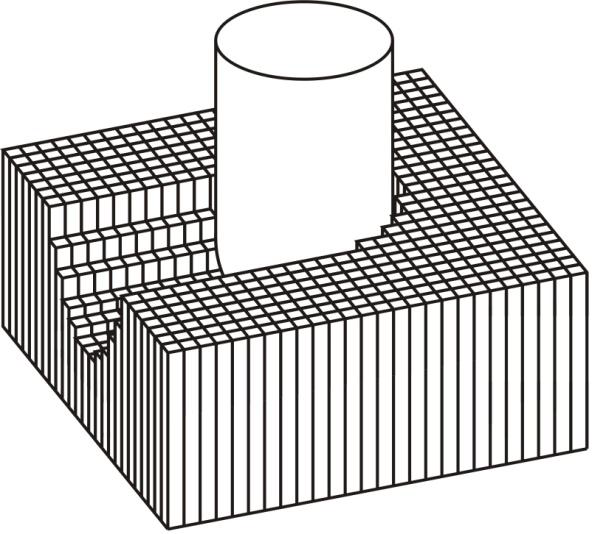
\includegraphics[width=\textwidth]{images/zmap}
			\caption{Prism representation of a z-map}
			\label{fig:zmap}
		\end{subfigure}
		\begin{subfigure}{0.4\textwidth}
			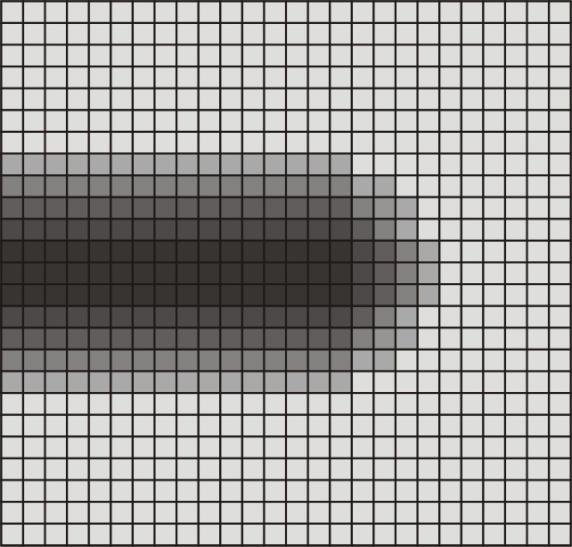
\includegraphics[width=\textwidth]{images/depth_image}
			\caption{depth image}
			\label{fig:depth_image}
		\end{subfigure}
		\caption{
			Representation of a cuboid stock with material removed using a ball-end cutter.
			The geometry described by the z-map is represented using right square prisms in the left image.
			The z-map can be stored in a grayscale image as shown on the right.
			Images by Tukora \cite{virtual_machining_review}.
		}
	\end{figure}
	
	\item[Dexel images]
	Dexel based representations have been proposed by Hook to circumvent the shortcomings of depth images \cite{dexel}.
	Instead of a scalar value per pixel of a regular 2-dimensional grid (z-maps) a complex data element is storing called dexel (abbreviated from depth element).
	A dexel is created by tracing a ray starting at a grid point perpendicular to the grid's plane through the workpiece and collecting all surface intersections.
	Each dexel stores a sorted list of these intersections, where an intersection is also called a dexel node.
	A node basically contains the depth value of the intersection and can contain further informations such as a surface normal or a color value.
	Pairs of dexel nodes where the first node has been an entry and the second an exit are called segments and always lie inside the workpiece.
	
	Material removal is done in a similar fashion as with with z-maps.
	A dexel image is created for a sweep and then combined with the dexel image of the current workpiece.
	Instead of updating to the minimum value as 
		
	\begin{figure}[h]
		\centering
		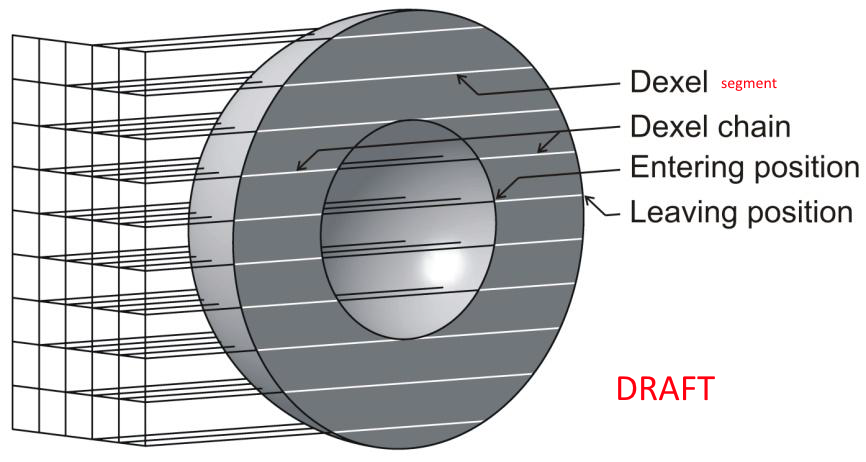
\includegraphics[width=\textwidth]{images/dexels}
		\caption{
			Dexel image for a half sphere with a smaller, concentric half sphere drilled out.
			Image adapted from Tukora \cite{virtual_machining_review}.
		}
		\label{fig:dexel_image}
	\end{figure}
		
	\item[Multi-dexel images]
	To increase the accuracy of dexel based models, especially 

	\begin{figure}
		\centering
		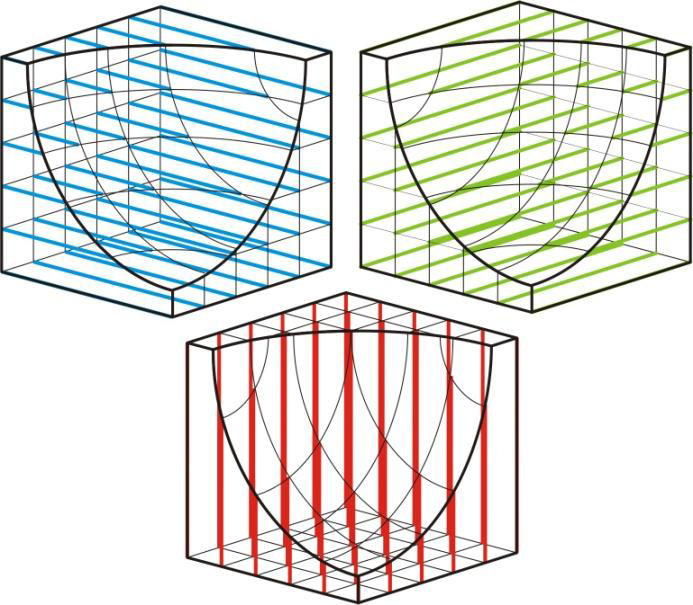
\includegraphics[width=\textwidth]{images/tridexels}
		\caption{Tri-dexel images}
		\label{fig:tri_dexel_image}
	\end{figure}

	\item[Constructive Solid Geometry (CSG)]
	
	\item[Uniform spacial decomposition (USD)]
	
	\item[Hierarchical spacial decomposition (HSD)]
	
	\item[Boundary representation (BRep)]
	
\end{description}

Implicit models may be composed of polygons, parametric surfaces and functional representations (iso surfaces).

Furthermore, many and also different types of such surfaces may be aggregated, referred to as B-rep (boundary representation), or combined using set operations such as in CSG.



\section{Triangulations}
\label{sec:definitions}

\begin{description}
	\item[Triangulation/Tesselation]
	
	\item[Mesh]
	
	\item[Manifold]
	
	\item[Oriented]
	
	\item[Closed/water-tight]
	
	\item[Boundary]
	
	\item[Voronoi]
	
	\item[Delaunay]
	A triangulation is called Delaunay when the circumcircle of each triangle does not contain a vertex of another triangle.
	Delaunay triangulations produce very regular and visually appealing triangle meshes.
	
	\item[Gabriel 2-Simplex]
	
	\item[Chord error]
	
\end{description}


\section{Surface reconstruction}
\label{sec:surface_reconstruction}

where is surface reconstruction used?
